
\def\rfdatascale{0.6}
\colorlet{h0}{red}
\colorlet{h1}{blue}
\colorlet{h2}{green!60!black!90}
\colorlet{fileheader}{gray!40!black!70}
  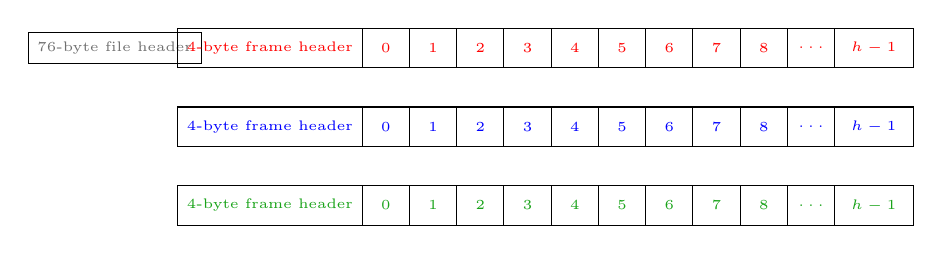
\begin{tikzpicture}
    [sample/.style={anchor=east,font=\tiny,minimum width=\rfdatascale cm,minimum height=.5cm,draw},
      hmax/.style={sample,anchor=west,minimum width=1cm}]
    
    \node[font=\tiny,draw] at (-3.75cm,3) {\color{fileheader}76-byte file header};
    
    \def\slabel{{\ifnum\x=-1{4-byte frame header} %
        \else\ifnum\x=9{$\ldots$} %
        \else\x\fi\fi}} %
    \foreach \x in {-1,0,1,...,8,9} {
      \node[sample] (p3\x) at (\rfdatascale*\x cm,3) {\color{h0}{\slabel}};
      \node[sample] (p2\x) at (\rfdatascale*\x cm,2) {\color{h1}{\slabel}};
      \node[sample] (p1\x) at (\rfdatascale*\x cm,1) {\color{h2}{\slabel}};
    }
    \node[hmax] [right of=p39,xshift=-.2cm] {\color{h0}$h-1$};
    \node[hmax] [right of=p29,xshift=-.2cm] {\color{h1}$h-1$};
    \node[hmax] [right of=p19,xshift=-.2cm] {\color{h2}$h-1$};
    
    \end{tikzpicture}


  
